\documentclass{ltxdoc}

\def\fileversion{0.1}
\def\filedate{2017/09/05}

\title{The \textsf{limecv} document class\thanks{This document corresponds to \textsf{limecv}~\fileversion, dated \filedate.}}

\author{Olivier Pieters \\ \texttt{me (at) olivierpieters (dot) be}}

\usepackage{listings}
\usepackage{tikz}
\usepackage{hyperref}

\usepackage{cleveref}
\usepackage{xparse}

\lstset{%
  basicstyle=\ttfamily, % font style and size
  breakatwhitespace=false,
  breaklines=true,
  numbers=left,
  numberstyle=\tiny,
  numbersep=5pt,
  language=[LaTeX]{TeX},
  keywordstyle=\color{blue},
  commentstyle=\color{red}
}

\NewDocumentCommand{\cvRequirement}{m}{\textbf{#1}}

\begin{document}

\maketitle

\tableofcontents

\section{Introduction}

This document class is designed to facilitate easy development of curriculum vit\ae\ (CV) with this particular design. Special elements have been designed of particular sections to ease quick creation. This document class was co-designed with a business card, which can be found on GitHub: \url{https://github.com/opieters/business-card}.

The design of this CV is split up in three parts, illustated by \cref{design}. Each of these parts that make up this CV template, will be detailed in the sections below.

\begin{figure}[!ht]
  \centering
  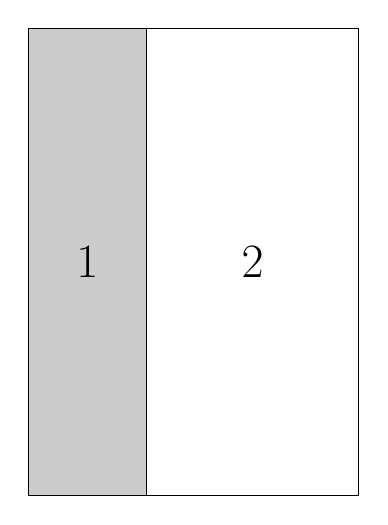
\begin{tikzpicture}
    \draw (0,0) rectangle ++(4.20,5.94);
    \draw[fill=black!20] (0,0) rectangle ++(1.5,5.94);
    \draw (0.75,2.97) node {\LARGE 1};
    \draw (2.85,2.97) node {\LARGE 2};
  \end{tikzpicture}%
  \hspace{2cm}%
  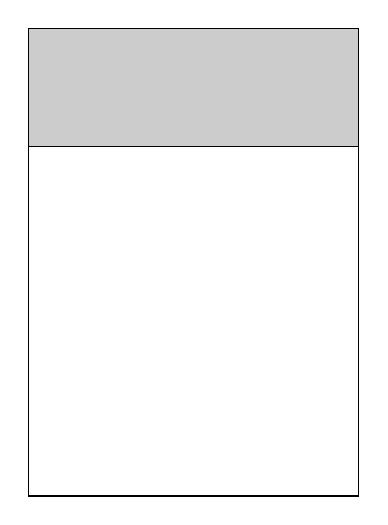
\begin{tikzpicture}
    \draw (0,0) rectangle ++(-4.20,-5.94);
    \draw[fill=black!20] (0,0) rectangle ++(-4.2,-1.5);
  \end{tikzpicture}
  \caption{Illustation of basic template. The left image depicts the actual CV: side bar to the left (1) with main content on the right (2). The right image depicts the cover letter design.}
  \label{design}
\end{figure}

\section{Requirements}

  Currently, it is advised to use the \cvRequirement{XeLaTeX} compiler. LaTeX will also work, but in that case icons are not available. In the subsequent, it will always be assumed that the XeLaTeX compiler is used (unless noted otherwise). 

  Any font can be used, though by default the \cvRequirement{Fira}\footnote{\url{https://github.com/mozilla/Fira}} font is used. This should be installed and accessable by the typesetting system. If another font is desired, it can be overwritten using the \lstinline|customfont| document class options and |\cvMainFont| command. 

  \cvRequirement{FontAwesome}\footnote{\url{http://fontawesome.io}} is the icon font used. This font should also be available and cannot be replaced by another icon font. 

\section{General Macros and Document Class Options}

\section{Side Bar}

  The side bar should contain personal information such as your name, job title (or industry or similar), contact information, small bio, interests and language skills. Special environments and commands have been defined for each of these sections and will be described below. 

  Everything that should be inside the side bar should be placed in the |cvSideBar| environment. This environment is placed on the left side of the page by default. If it should be typeset on the right side, use the starred version (|cvSideBar*|)

  The following environments are available inside the side bar environment: |cvProfile|, |cvContact|, |cvLanguages|, |cvInterests| and |cvProjects|.
  
  \DescribeMacro{\cvID}
  This command typesets a picture (in a circle) with name and position underneath it.
  The argument order is: |\cvID{|\meta{first name}|}{|\meta{last name}|}{|\meta{picture location}|}{|\meta{job position}|}|. Empty fields are allowed for the third and fourth arguments. No picture and no job position will then be typeset. Example code: 
  \begin{lstlisting}
\cvID{John}{Doe}{profile_picture}{Broaker}
  \end{lstlisting}
  
  \DescribeMacro{cvProfile} 
  This environment contains a brief profile description or biography. No additional arguments are allowed. Example code:
  \begin{lstlisting}
\begin{cvProfile}
  A short biography goes here.
\end{cvProfile}
  \end{lstlisting}
  
  \DescribeMacro{cvContact} 
  All the contact information goes here. Inside this environment, the following commands are available: 
  \begin{itemize}
    \item \DescribeMacro{\cvContactAddress} |\cvContactAddress{|\meta{address}|}| typesets an address. How this address should be typeset exactly is left to the user. The use of line breaks (|\\|) is allowed;
    \item \DescribeMacro{\cvContactEmail} |\cvContactEmail{|\meta{link}|}{|\meta{email address}|}| typesets an email address. The link variable should be a something like |mailto:john@doe.tld|. Clicking on the email address will then automatically open the default email client with this address as recipient. If the link argument is left empty, no link will be created. 
    \item \DescribeMacro{\cvContactPhone} |\cvContactPhone{|\meta{mobile phone number}|}| typesets a mobile phone number.
    \item \DescribeMacro{\cvContactWebsite} |\cvContactWebsite{|\meta{link}|}{|\meta{website URL}|}| typesets a website. The link variable should be a something like |https://johndoe.tld|. Clicking on the website will then automatically open the default web browser. If the link argument is left empty, no action will be performed upon clicking on the website.
    \item \DescribeMacro{\cvContactGithub} |\cvContactGithub{|\meta{link}|}{|\meta{username}|}| typesets a GitHub profile. The link variable should be a valid link to the GitHub profile (for example |https://github.com/johndoe|). Clicking on the username will then automatically open the default web browser. If the link argument is left empty, no action will be performed upon clicking on the website.
    \item \DescribeMacro{\cvContactLinkedin} |\cvContactLinkedin{|\meta{link}|}{|\meta{username}|}| typesets a LinkedIn profile. The link variable should be a link to your LinkedIn profile homepage (for example |https://www.linkedin.com/in/johndoe/|). Clicking on the username will then automatically open the default web browser. If the link argument is left empty, no action will be performed upon clicking on the website. 
    \item \DescribeMacro{\cvContactTwitter} |\cvContactTwitter{|\meta{link}|}{|\meta{username}|}| typesets a Twitter profile. The link variable should direct to your Twitter profile. An example link looks as follows: |https://twitter.com/johndoe|. Clicking on the username will then automatically open the default web browser. If the link argument is left empty, no action will be performed upon clicking on the website.this address as recipient. If the link argument is left empty, no link will be created. 
    \item \DescribeMacro{\cvContactKeybase} |\cvContactKeybase{|\meta{link}|}{|\meta{fingerprint}|}| typesets a keybase fingerprint (and account). The link variable should be a link to the KeyBase profile (e.g.\ |https://keybase.io/johndoe|). Clicking on the fingerprint will then automatically open the default web browser. If the link argument is left empty, no action will be performed upon clicking on the website.
  \end{itemize}
  
  A full example:
  \begin{lstlisting}
\begin{cvContact}
  \cvContactAddress{Some Street 78\\B-9000 Ghent\\Belgium}
  \cvContactEmail{mailto:john@doe.tld}{john@doe.tld}
  \cvContactPhone{+1 781 555 1212}
  \cvContactWebsite{https://doe.tld}{doe.tld}
  \cvContactGithub{https://github.com/johndoe}{johndoe}
  \cvContactLinkedin{https://www.linkedin.com/in/johndoe/}{johndoe}
  \cvContactTwitter{https://twitter.com/johndoe}{@johndoe}
  \cvContactKeybase{https://keybase.io/johndoe}{\texttt{AAAA 5555 BBBB FFFF}}
\end{cvContact}
  \end{lstlisting}

  If you wish to add contact information that is not available by default, you can extend the command using two internal commands: |\cv@ContactTemplateLink| and |\cv@ContactTemplate|. See the source code for usage instructions.

  \DescribeMacro{cvLanguages} This environment is used to showcase language skills. The \DescribeMacro{\cvLanguage} |\cvLanguage{|\meta{language}|}{|\meta{skill level}|}| should be used inside this environment. The skill level is a real value with a maximum value of 5. If higher values are used, the result will not be typeset properly. An example is included below.

  \begin{lstlisting}
\begin{cvLanguages}
  \cvLanguage{English (native)}{5}
  \cvLanguage{German (B1)}{3}
  \cvLanguage{Spanish}{3}
\end{cvLanguages}  
  \end{lstlisting}

  \DescribeMacro{cvInterests} Typeset interests (can be both professional and personal) using |cvInterests|. By default it just typesets a list of items in the long format (|long|). The short format can be activated by passing the |short| option to the environment. Inside this environment, three commands can be used: |\cvInterestsPersonal|, |\cvInterestsProfessional| and |\cvInterest|. \DescribeMacro{\cvInterestsPersonal} |\cvInterestsPersonal| and \DescribeMacro{\cvInterestsProfessional} |\cvInterestsProfessional| add optional sections inside this environment to differentiate between personal and professional interests respectively. Both macros have no options nor arguments. The \DescribeMacro{\cvInterest} |\cvInterest{|\meta{icon}|}{|\meta{interest}|}| command takes an icon and interest as arguments. Note that if \LaTeX\ is used, the icon argument will be ignored. In this case, there is also no difference between the |long| and |short| options of the |cvInterests| environment.
  
  Examples that illustrate the different options are depicted below:

  \begin{lstlisting}
\begin{cvInterests}
  \cvInterestsPersonal
  \cvInterest{\faTrain}{model trains}
  \cvInterest{\faFlask}{(applied) sciences}
  \cvInterest{\faSuitcase}{travelling}
  \cvInterestsProfessional
  \cvInterest{\faGraduationCap}{machine learning}
  \cvInterest{\faMicrochip}{electronics}
  \cvInterest{\faCogs}{robotics}
\end{cvInterests}
  \end{lstlisting}
  
  \begin{lstlisting}
\begin{cvInterests}[short]
  \cvInterestsPersonal
  \cvInterest{\faTrain}{model trains}
  \cvInterest{\faFlask}{(applied) sciences}
  \cvInterest{\faSuitcase}{travelling}
  \cvInterest{\faCamera}{photography}
  \cvInterest{\faGamepad}{gaming}
  \cvInterest{\faMusic}{music}
\end{cvInterests}
  \end{lstlisting}
  
  \DescribeMacro{cvProjects} If you have interesting (side) projects that are relevant for your CV, you can list them using the |cvProjects| environment. Inside this environment you can use the \DescribeMacro{\cvProject} |\cvProject[|\meta{options}|]{|\meta{name}|}{|\meta{description}|}| macro to list all your projects. The only options currently allowed in \meta{options} are to pass an image (using |image|) and a URL (using |link|). This image must be an external file and the user must handle its size through |width| or |height|. Example usage:
  
  \begin{lstlisting}
\begin{cvProjects}
  \cvProject[image=clock,width=1cm]{yanic}{An IoT nixie clock.}
  \cvProject{\texttt{limecv}}{A \LaTeX\ document class for curriculum vit\ae.}
\end{cvProjects}
  \end{lstlisting}
  
  It is currently not possible to extend the side bar with additional environments. To add your own, look at the source code and create your own \LaTeX-style hack.  

\section{Main Content}

  The main content section includes details on your education, experience, skills, references and more. Several environments have been designed to suit specific needs. These will be discussed next.
  
  \DescribeMacro{cvMainContent} 
  Everything in the main content section should be encapsulated in the |cvMainContent| environment. This environment defines four new environments: |cvEducation|, |cvExperience|, |cvSkills| and |cvReferences|. These four environments are self explanatory in terms of function. Subsequently, we will detail each of these environments.
  
  Note that |cvMainContent| also has a starred variant (|cvMainContent*|). The function is similar to |cvSideBar*|, in the sense that it places everything to the left instead of the default right location.
  
  \DescribeMacro{cvEducation} 
  The education environment creates a timeline styled list of your education. Individual education items should be listed by means of the |\cvItem{|\meta{details}|}| macro which is available within this environment. Instead of forcing a specific layout structure, it was preferred to leave the actual markup to the end user. \emph{All} information concerning a single education should be passed to this single argument. However, the user is always welcome to create his own styling macro that takes multiple arguments. This is illustrated by the examples below.
  
  \begin{lstlisting}[caption={\lstinline!cvEducation! \emph{without} special user markup command.}]
\begin{cvEducation}
  \cvItem{Evening class: Chinese\\
  Some School, City. September 2015 -- June 2016\\
  Achieved A2 language skill in Chinese (Mandarin).}
  \cvItem{Bachelor of Science in Biochemistry and Biotechnology\\
  University, City. September 2009 -- June 2012\\
  General training in the basic sciences and the molecular life science.}
  \cvItem{Master of Science in Biochemistry and Biotechnology\\
  University, City. September 2012 -- June 2015\\
  Acquisition of insight into and knowledge of possibilities for application in the area of biochemistry and biotechnology, specific with applications in biomedical application and due problem-solving reasoning skills.}
\end{cvEducation}
  \end{lstlisting}
  
  \begin{lstlisting}[caption={\lstinline!cvEducation! \emph{with} special user markup command.}]
% in preamble:
\newfontfamily\firaMedium{Fira Sans Medium}
\NewDocumentCommand{\cvEducation}{mmm}{{\firaMedium #1}\\ #2\\ \emph{#3}}
% in document:
\begin{cvEducation}
  \cvItem{\cvEducation{Evening class: Chinese}%
            {Some School, City. September 2015 -- June 2016}%
            {Achieved A2 language skill in Chinese (Mandarin).}}
  \cvItem{\cvEducation{Bachelor of Science in Biochemistry and Biotechnology}%
            {University, City. September 2009 -- June 2012}%
            {General training in the basic sciences and the molecular life science.}}
  \cvItem{\cvEducation{Master of Science in Biochemistry and Biotechnology}%
            {University, City. September 2012 -- June 2015}%
            {Acquisition of insight into and knowledge of possibilities for application in the area of biochemistry and biotechnology, specific with applications in biomedical application and due problem-solving reasoning skills.}}
\end{cvEducation}
  \end{lstlisting}
  
  \DescribeMacro{cvExperience} 
  |cvExperience| works very similar to |cvEducation|. If follows the exact same structure and has the same design philosophy where you should use |\cvItem| inside this environment to typeset the individual items in a timeline style. \Cref{} illustrates this with an example.

  \begin{lstlisting}[caption={\lstinline!cvExperience! code example.}]
\begin{cvExperience}
  \cvItem{Student Job\\
    \textsc{\selectfont Company X}, Location X. Summer 2010\\
    Integer tincidunt dapibus consectetur. Nullam tristique aliquam luctus. Sed ut ante velit. Nulla pharetra maximus lacus at elementum. Suspendisse sodales consectetur metus, sit amet ultricies ipsum ultrices ut.};
  \cvItem{Internship\\
    \textsc{Company Y}, Location Y. June 2012 -- August 2012\\
     Lorem ipsum dolor sit amet, consectetur adipiscing elit. Morbi dictum cursus sapien, id eleifend mi pellentesque id. Etiam lobortis eu odio a sodales. Phasellus ut dolor feugiat, lacinia lectus in, blandit metus. Fusce lacinia dolor et metus gravida pulvinar sit amet et ex.};
  \cvItem{Internship\\
    \textsc{Company Z}, Location Z. August 2014 -- September 2014\\
    Lorem ipsum dolor sit amet, consectetur adipiscing elit. Morbi dictum cursus sapien, id eleifend mi pellentesque id. Etiam lobortis eu odio a sodales. Phasellus ut dolor feugiat, lacinia lectus in, blandit metus.  Fusce lacinia dolor et metus gravida pulvinar sit amet et ex. Suspendisse vestibulum, leo malesuada molestie maximus, sem risus ornare elit, vitae sodales felis elit in ipsum.};
\end{cvExperience}
  \end{lstlisting}
  
  \DescribeMacro{cvSkills} 
  The skills section is contained within the |cvSkills| environment. This environment typesets your skills on a 5-level (discrete) scale (with the default |dot| option) or a 5-level continuous scale with the |bar| option. These are divided in two columns. To that end, two macros are available: |cvSkillOne| and |cvSkillTwo|. \DescribeMacro{cvSkillTwo} |cvSkillTwo{|\meta{skill level}|}{|\meta{skill}|}{|\meta{skill level}|}{|\meta{skill}|}| typesets a row of two skills. If you have an odd number of items, \DescribeMacro{cvSkillOne} |cvSkillOne| should be used. An example of a skill-list can be found in \cref{cvSkills}.
  
  \begin{lstlisting}[caption={Illustration of the \lstinline!cvSkills! environment.},label=cvSkills]
\begin{cvSkills}
  \cvSkillTwo{5}{MATLAB}{5}{\LaTeX}
  \cvSkillTwo{4}{Python}{4}{VHDL}
  \cvSkillTwo{4}{Microsoft Office}{4}{macOS}
  \cvSkillOne{3}{C, C++}
\end{cvSkills}
  \end{lstlisting}
  
  \DescribeMacro{cvReferences}
  The final section is intended to list all your references. These go inside the |cvReferences| environment. The enumeration of the different items should be done using the \DescribeMacro{\cvAddReference} |\cvAddReference{|\meta{information}|}| macro. The following keys are available: |name|, |company|, |job|, |address line 1|, |address line 2|, |address line 3|, |mobile phone|, |work phone| and |email|. These are all optional arguments and will be typeset consistently between the two references per row. If icons are undesirable, use the |noicon| option for the environment. \Cref{cvReferences} illustrates the usage of this environment.
  
  \emph{Important remark}: the comment after the usage of |\cvAddReference| is required! Otherwise, spacing will not be as designed.
  
  \begin{lstlisting}[caption={\lstinline!cvReferences! code example.},label=cvReferences]
\begin{cvReferences}
  \cvAddReference{%
    name=Jane Smith,
    company=Company ABC Co.\ Ltd.,
    job=Job title,
    address line 1=Street lane 2,
    address line 2=B-1150 Brussels,
    mobile phone=+1 781 555 1212}% <<-- Important!!!
\end{cvReferences}
  \end{lstlisting}

\section{Cover Letter}

  A final (optional) part of a CV is the cover letter. This is a fairly simple part to create design wise, but probably the hardest to write in an actual CV. 

  \DescribeMacro{cvCoverLetter}
  The cover letter environment is |cvCoverLetter| and contains all the cover letter details. It will automatically add a header with your name and position based on the information filled in in |\cvID|. 
  
  \DescribeMacro{\cvBeneficiary}
  The |\cvBeneficiary{|\meta{options}|}| macro offers a convenience wrapper to typeset the beneficiary. Possible options are |name|, |position|, |company|, |address line 1|, |address line 2| and |address line 3|. The remainder of the cover letter design is up to the user. An example design can be found in \cref{cvCoverLetter}.
  
  \DescribeMacro{\cvFullName}
  |\cvFullName| typeset the authors name based on the data provided in |cvID|. 

  \begin{lstlisting}[caption={\lstinline!cvCoverLetter! code example.},label=cvCoverLetter]
\section{Cover Letter}

\begin{cvCoverLetter}

\cvBeneficiary{%
  name=Jane Smith,
  position=Position,
  company=Company,
  address line 1=Address line 1,
  address line 2=Address line 2}

Dear Miss.\ Smith

\vspace{\baselineskip}
\lipsum[1-3]
\vspace{\margin}

\cvFullName

\end{cvCoverLetter}
  \end{lstlisting}

\section{Example}

  The source code of a typical CV document can be found below. \Cref{example-cv,example-cover-letter} depict the resulting PDF documents.

  \begin{figure}[!ht]
    \includegraphics[width=\textwidth,page=1]{mwe.pdf}
    \caption{Example CV (scaled).}
    \label{example-cv}
  \end{figure}

  \begin{figure}[!ht]
    \includegraphics[width=\textwidth,page=2]{mwe.pdf}
    \caption{Example cover letter (scaled).}
    \label{example-cover-letter}
  \end{figure}

  \lstinputlisting[language=tex]{mwe.tex}

\section{Source Code}

\lstinputlisting[language=tex]{limecv.cls}

\PrintIndex

\end{document}